% Arquitectura de MARLUP (prealimentación pura). Compilar con: pdflatex fig3_cascada.tex
% Simétrica respecto del centro: cinemática inversa y plataforma a la misma distancia de los actuadores,
% y el oleaje centrado debajo, con sus dos salidas simétricas.
\documentclass[tikz,border=4pt]{standalone}
\usepackage[T1]{fontenc}
\usepackage{newtxtext,newtxmath}
\usepackage{amsmath}
\usepackage{siunitx}
\usetikzlibrary{positioning,arrows.meta,calc,fit,backgrounds}

\begin{document}
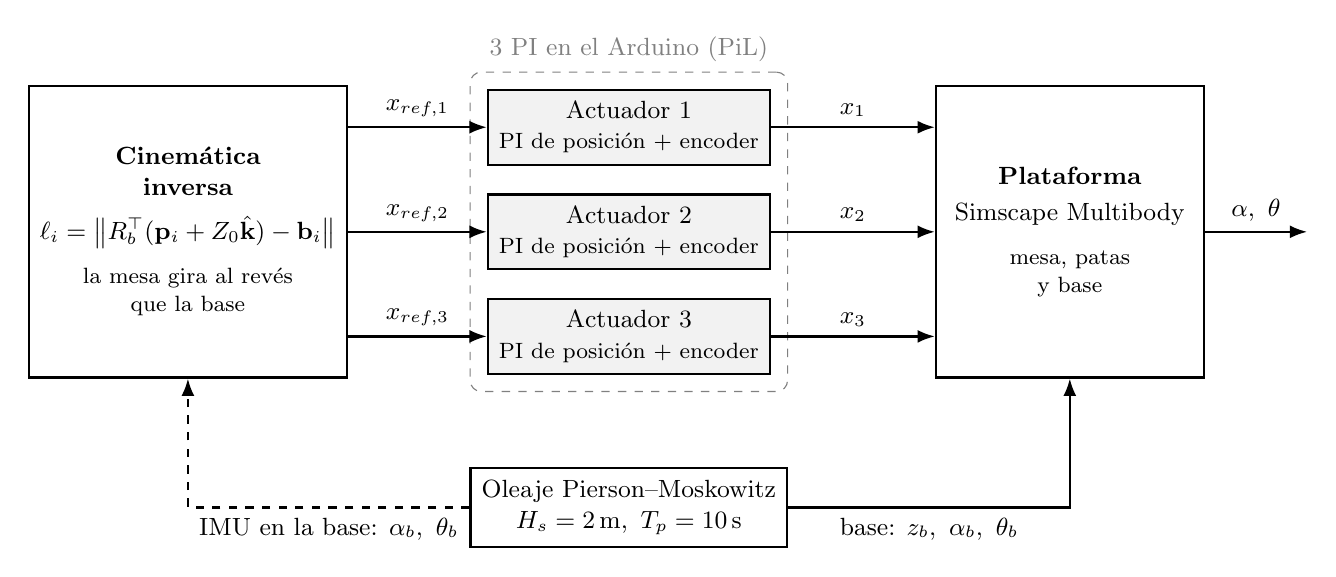
\begin{tikzpicture}[
    >={Latex[length=2.2mm]},
    font=\small,
    blk/.style={draw, thick, align=center, inner sep=4pt},
    act/.style={blk, fill=black!5, minimum width=3.0cm, minimum height=0.95cm},
    sig/.style={->, thick},
    dsig/.style={->, thick, dashed},
  ]
  \def\D{5.6}      % distancia del centro a la cinemática y a la plataforma
  \def\W{3.4cm}    % ancho común de ambos bloques
  \def\H{3.7cm}    % alto común

  % ---------------- actuadores (centro) ----------------
  \node[act] (a2) at (0,0) {Actuador 2\\ \footnotesize PI de posición + encoder};
  \node[act, above=0.35cm of a2] (a1) {Actuador 1\\ \footnotesize PI de posición + encoder};
  \node[act, below=0.35cm of a2] (a3) {Actuador 3\\ \footnotesize PI de posición + encoder};
  \begin{scope}[on background layer]
    \node[draw, dashed, gray, rounded corners, inner sep=6pt, fit=(a1)(a3),
          label={[gray]above:{3 PI en el Arduino (PiL)}}] (pil) {};
  \end{scope}

  % ---------------- cinemática inversa y plataforma (simétricas) ----------------
  \node[blk, minimum width=\W, minimum height=\H] (ik) at (-\D,0)
       {\textbf{Cinemática}\\ \textbf{inversa}\\[5pt]
        $\ell_i=\big\lVert R_b^{\top}(\mathbf{p}_i+Z_0\hat{\mathbf{k}})-\mathbf{b}_i\big\rVert$\\[5pt]
        \footnotesize la mesa gira al revés\\[-1pt] \footnotesize que la base};
  \node[blk, minimum width=\W, minimum height=\H] (plat) at (\D,0)
       {\textbf{Plataforma}\\[2pt] Simscape Multibody\\[5pt] \footnotesize mesa, patas\\[-1pt] \footnotesize y base};

  \foreach \i in {1,2,3} {
    \draw[sig] (ik.east |- a\i.west) -- node[above] {$x_{ref,\i}$} (a\i.west);
    \draw[sig] (a\i.east) -- node[above] {$x_{\i}$} (a\i.east -| plat.west);
  }
  \draw[sig] (plat.east) -- node[above] {$\alpha,\ \theta$} ++(1.3,0);

  % ---------------- oleaje, centrado debajo, con salidas simétricas ----------------
  \node[blk, minimum width=3.6cm, minimum height=1.0cm] (ola) at (0,-3.5)
       {Oleaje Pierson--Moskowitz\\ $H_s=\SI{2}{m},\ T_p=\SI{10}{s}$};
  \draw[dsig] (ola.west) -| node[pos=0.25, below] {IMU en la base: $\alpha_b,\ \theta_b$} (ik.south);
  \draw[sig] (ola.east) -| node[pos=0.25, below] {base: $z_b,\ \alpha_b,\ \theta_b$} (plat.south);

\end{tikzpicture}
\end{document}
